\section{Gráficos e análise dos dados}

Os gráficos foram gerados usando o LibreOffice Calc.
% %GRAFICO 1

\subsection{Média do Tempo Total de Execução Dos Testes}

O tempo total de execução do teste tem como finalidade mostrar o tempo em que o 
processo do ApacheBench responsável pelo teste ficou em execução no sistema 
operacional. Tendo em vista que o processo do ApacheBench pode ficar em 
execução 
por mais tempo do que a realização do teste e que uma requisição pode demorar a 
responder, atrasando o fim do teste, essa métrica provê uma noção do desempenho 
do servidor, mais não deve ser levado em consideração em uma análise adequada. 
No caso desta métrica, quanto menor o valor observado, melhor.

\begin{figure}[H]
	\centering
	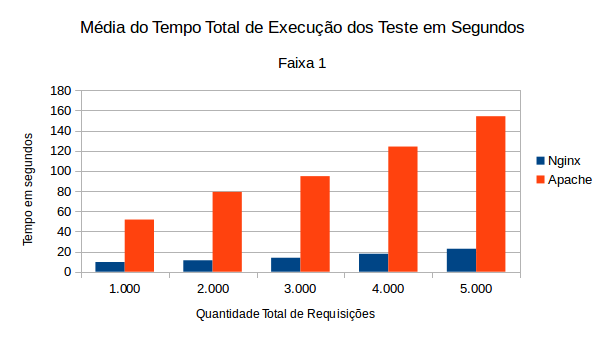
\includegraphics[width=1\linewidth]{graficos/grafico1-f1} 
	\caption{Média do Tempo Total de Execução dos Testes - Faixa 1}
	\label{fig:grafico1-f1}
\end{figure}

\begin{figure}[H]
	\centering
	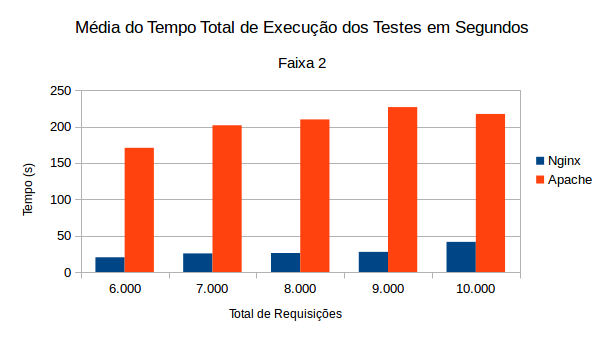
\includegraphics[width=1\linewidth]{graficos/grafico1-f2} 
	\caption{Média do Tempo Total de Execução dos Testes - Faixa 2}
	\label{fig:grafico1-f2}
\end{figure}

\begin{figure}[H]
	\centering
	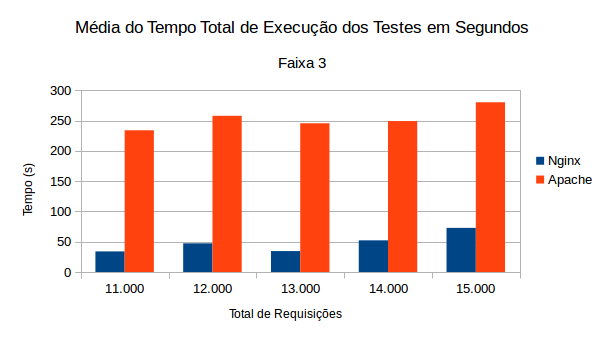
\includegraphics[width=1\linewidth]{graficos/grafico1-f3} 
	\caption{Média do Tempo Total de Execução dos Testes - Faixa 3}
	\label{fig:grafico1-f3}
\end{figure}

\begin{figure}[H]
	\centering
	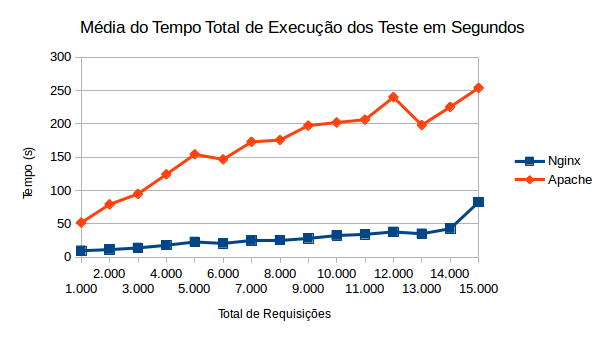
\includegraphics[width=1\linewidth]{graficos/grafico1} 
	\caption{Média do Tempo Total de Execução dos Testes}
	\label{fig:grafico1}
\end{figure}

Ao analisar os resultados obtidos pelos testes, sob a Faixa 1, é possível ver 
que o servidor Apache demorou, em média 6,31 vezes mais do que no servidor 
Nginx. 
Na Faixa 2, os testes demoraram 7,57 vezes mais para serem executados no 
Apache. Na Faixa 3, os testes no Nginx demoraram, em média 5,61 vezes menos 
para serem executados.

Em termos gerais, levando em consideração os quinze valores de requisições 
totais, os tempos de execução dos testes no Apache foram em média 6,50 vezes 
mais lentos do que no Nginx. A soma dos tempos de totais dos testes foram: 
467,19 segundos para o Nginx contra 2.824,64 segundos para o Apache.
% %GRAFICO 2

\subsection{Média do Total de Dados Transferido}
O total de dados transferidos mostra a quantidade de informações que foram 
trocadas entre os computadores, incluindo os dados enviados pelas requisições e 
os dados retornados pelo servidor. Para fins de análise, os dados foram 
convertidos de bytes para Mega bytes. No caso desta métrica, quanto maior o 
valor observado, melhor.

\begin{figure}[H]
	\centering
	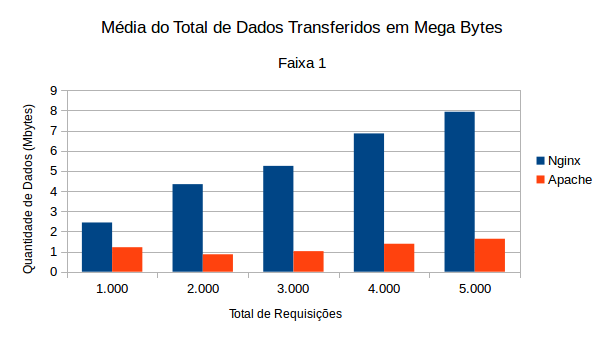
\includegraphics[width=1\linewidth]{graficos/grafico2-f1} 
	\caption{Média do Total de Dados Transferido - Faixa 1}
	\label{fig:grafico2-f1}
\end{figure}

\begin{figure}[H]
	\centering
	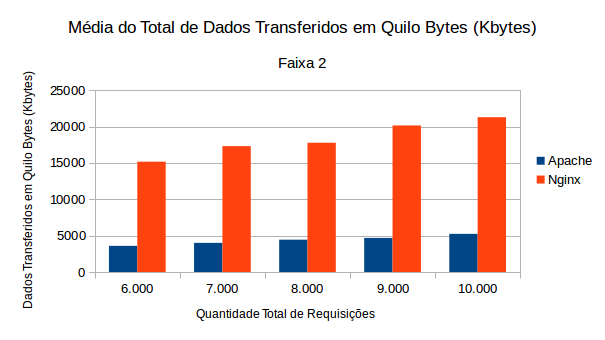
\includegraphics[width=1\linewidth]{graficos/grafico2-f2} 
	\caption{Média do Total de Dados Transferido - Faixa 2}
	\label{fig:grafico2-f2}
\end{figure}

\begin{figure}[H]
	\centering
	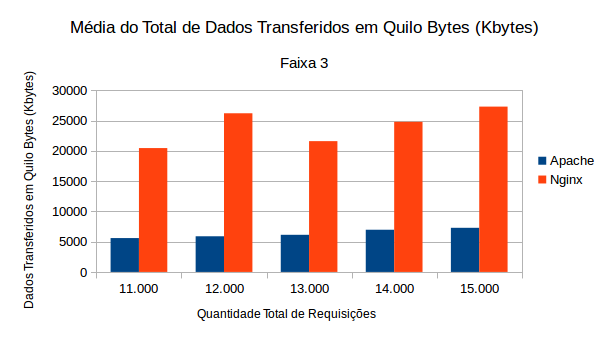
\includegraphics[width=1\linewidth]{graficos/grafico2-f3} 
	\caption{Média do Total de Dados Transferido - Faixa 3}
	\label{fig:grafico2-f3}
\end{figure}

\begin{figure}[H]
	\centering
	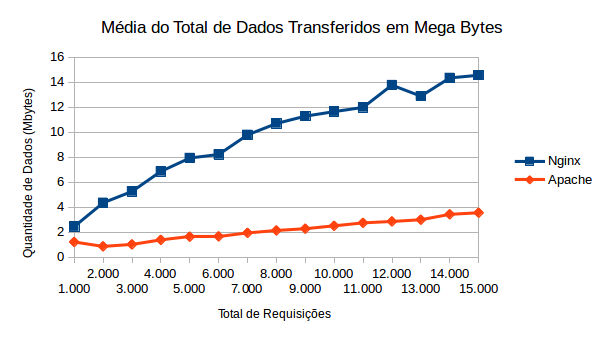
\includegraphics[width=1\linewidth]{graficos/grafico2} 
	\caption{Média do Total de Dados Transferido}
	\label{fig:grafico2}
\end{figure}

No geral, nos testes com o Nginx foram trafegados 4,55 vezes mais dados 
comparado com o Apache. Na Faixa 1, o Nginx obteve um desempenho 4,39 vezes 
superior em relação ao Apache. Nas Faixas 2 e 3, os resultados mostraram 
números semelhantes, apontando que o Nginx transferiu 4,91 vezes mais dados do 
que o Apache na Faixa 2 e 4,35 vezes mais dados do que o Apache na Faixa 3.
% %GRAFICO 3

\subsection{Média do Total de Texto HTML Transferido}

Ao se usar este indicador, é possível analisar a quantidade de páginas em HTML 
foram que retornados pelos servidores nos testes. Os números obtidos nessa 
métrica influenciam diretamente os dados coletados na métrica analisada 
anteriormente pelo fato de que, as páginas em HTML correspondem a maior parte 
do tráfego de dados entre o servidor e o cliente, respondendo por, em média, 
90\% dos dados. No caso desta métrica, quanto maior o valor observado, melhor.

\begin{figure}[H]
	\centering
	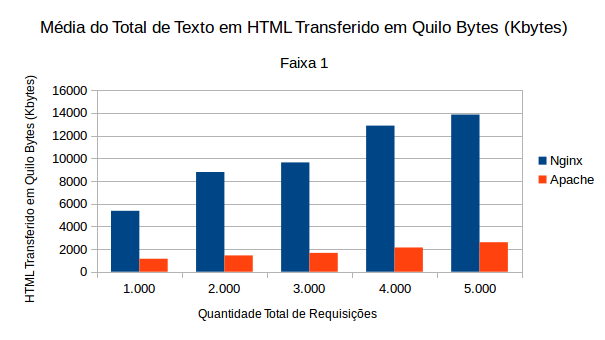
\includegraphics[width=1\linewidth]{graficos/grafico3-f1} 
	\caption{Média do Total de Texto HTML Transferido - Faixa 1}
	\label{fig:grafico3-f1}
\end{figure}

\begin{figure}[H]
	\centering
	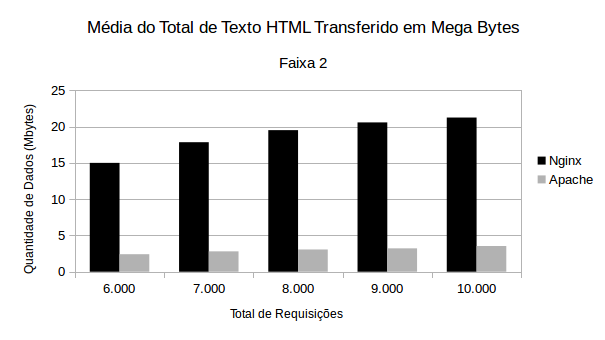
\includegraphics[width=1\linewidth]{graficos/grafico3-f2} 
	\caption{Média do Total de Texto HTML Transferido - Faixa 2}
	\label{fig:grafico3-f2}
\end{figure}

\begin{figure}[H]
	\centering
	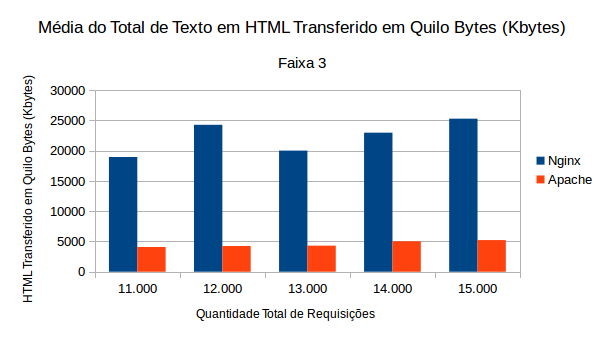
\includegraphics[width=1\linewidth]{graficos/grafico3-f3} 
	\caption{Média do Total de Texto HTML Transferido - Faixa 3}
	\label{fig:grafico3-f3}
\end{figure}

\begin{figure}[H]
	\centering
	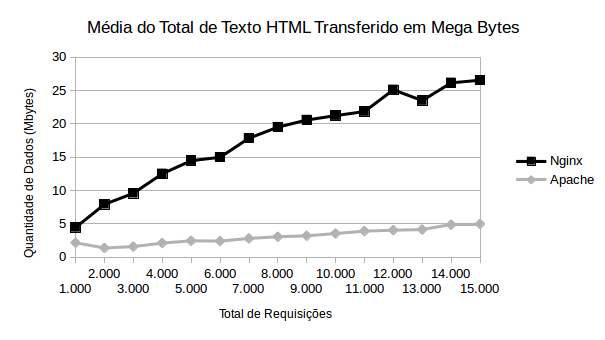
\includegraphics[width=1\linewidth]{graficos/grafico3} 
	\caption{Média do Total de Texto HTML Transferido}
	\label{fig:grafico3}
\end{figure}

O Nginx entregou, em média, 5,67 vezes mais dados em HTML do que o Apache. 
Analisando as faixas de valores de requisição, o Nginx conseguiu entregar na 
Faixa 1 5,12 vezes mais dados do que o Apache. Na Faixa 2, o desempenho do 
Nginx foi 6,26 vezes superior e na Faixa 3, 5,63 vezes superior ao Apache.
% %GRAFICO 4

\subsection{Média do Número de Requisições Atendidas}

Esse indicador é calculado de acordo com o tempo total gasto pela execução do 
teste e, como já falado, o tempo de execução do teste é uma métrica para 
auxiliar na análise do desempenho dos servidores. Assim sendo, o indicador de 
número do requisições atendidas também deve ser interpretado como um indicador 
auxiliar na análise de desempenho. No caso desta métrica, quanto maior o valor 
observado, melhor.

\begin{figure}[H]
	\centering
	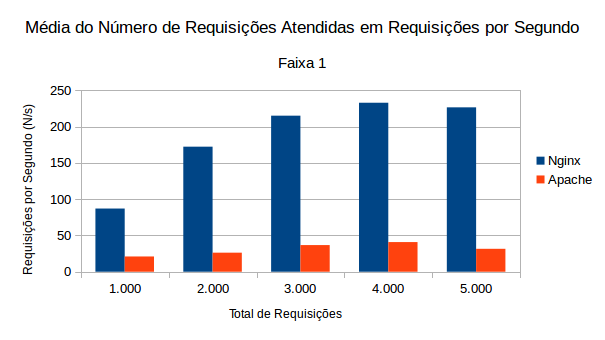
\includegraphics[width=1\linewidth]{graficos/grafico4-f1} 
	\caption{Média do Número de Requisições Atendidas - Faixa 1}
	\label{fig:grafico4-f1}
\end{figure}

\begin{figure}[H]
	\centering
	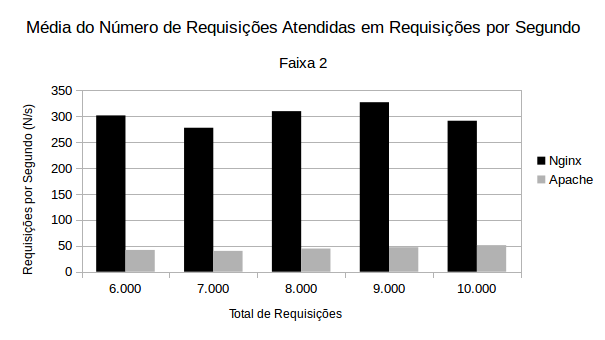
\includegraphics[width=1\linewidth]{graficos/grafico4-f2} 
	\caption{Média do Número de Requisições Atendidas - Faixa 2}
	\label{fig:grafico4-f2}
\end{figure}

\begin{figure}[H]
	\centering
	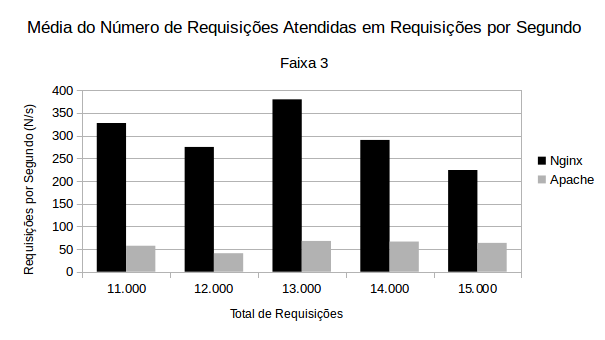
\includegraphics[width=1\linewidth]{graficos/grafico4-f3} 
	\caption{Média do Número de Requisições Atendidas - Faixa 3}
	\label{fig:grafico4-f3}
\end{figure}

\begin{figure}[H]
	\centering
	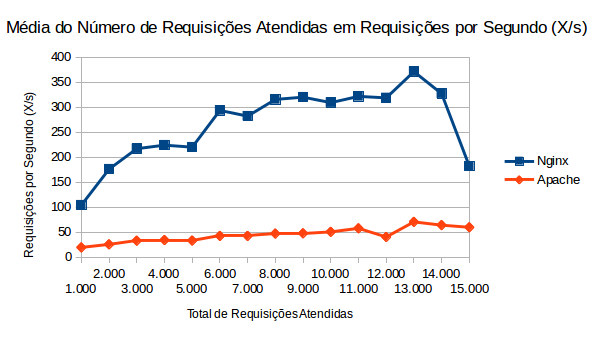
\includegraphics[width=1\linewidth]{graficos/grafico4} 
	\caption{Média do Número de Requisições Atendidas}
	\label{fig:grafico4}
\end{figure}

Ao analisar os dados e os gráficos vemos que o Nginx, no geral, obteve uma taxa 
de requisições atendidas por segundo 5,92 vezes maior do que o Apache. 
Analisando os gráficos e os dados das Faixas 1, 2 e 3, vemos que a taxa de 
requisições atendidas pelo Nginx é, na Faixa 1, 5,88 vezes superior ao Apache. 
Na Faixa 2 o desempenho é 6,71 vezes superior, e na Faixa 3, 5,18 vezes 
superior. 
% %GRAFICO 5

\subsection{Média do Tempo de Resposta por Requisição Simultânea}

Nessa métrica, foi calculado o tempo de resposta para as requisições que foram 
feitas de forma simultânea. Como essa métrica mede o tempo entre a emissão da 
requisição e a resposta do servidor, é uma métrica mais acurada para analisar o 
desempenho dos servidores nos testes. No caso desta métrica, quanto menor o 
valor observado, melhor.

\begin{figure}[H]
	\centering
	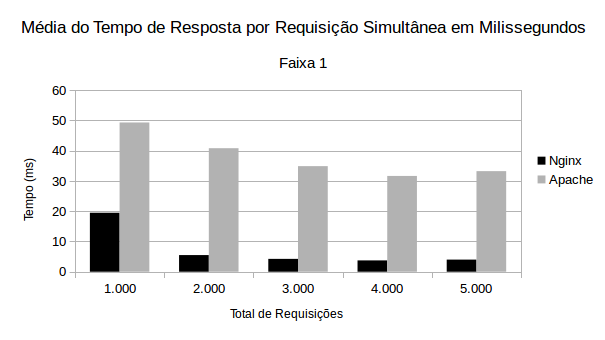
\includegraphics[width=1\linewidth]{graficos/grafico5-f1} 
	\caption{Média do Tempo de Resposta por Requisição Simultânea - Faixa 1}
	\label{fig:grafico5-f1}
\end{figure}

\begin{figure}[H]
	\centering
	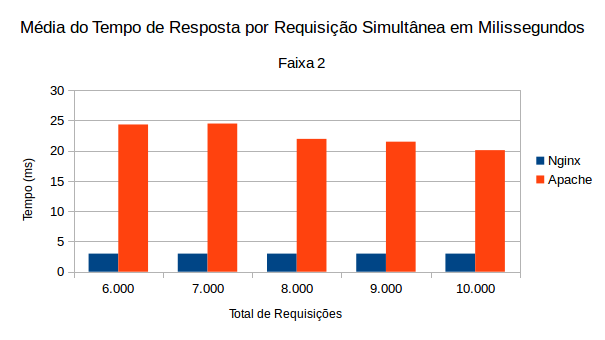
\includegraphics[width=1\linewidth]{graficos/grafico5-f2} 
	\caption{Média do Tempo de Resposta por Requisição Simultânea - Faixa 2}
	\label{fig:grafico5-f2}
\end{figure}

\begin{figure}[H]
	\centering
	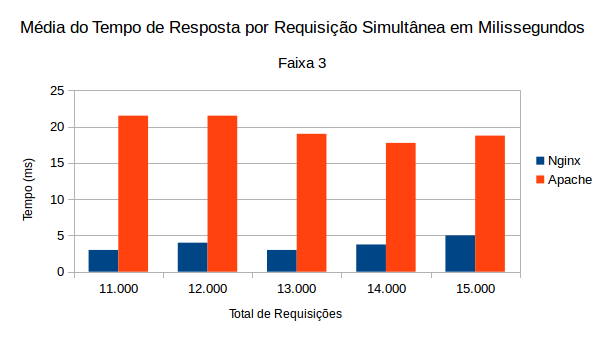
\includegraphics[width=1\linewidth]{graficos/grafico5-f3} 
	\caption{Média do Tempo de Resposta por Requisição Simultânea - Faixa 3}
	\label{fig:grafico5-f3}
\end{figure}

\begin{figure}[H]
	\centering
	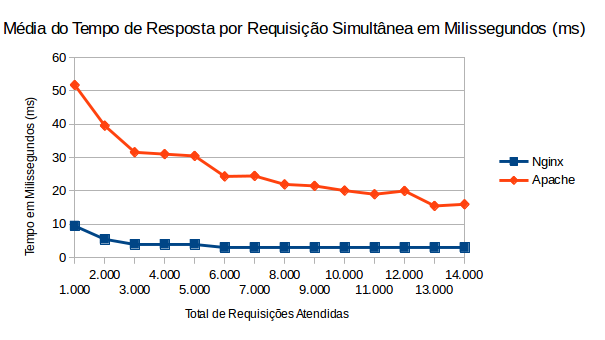
\includegraphics[width=1\linewidth]{graficos/grafico5} 
	\caption{Média do Tempo de Resposta por Requisição Simultânea}
	\label{fig:grafico5}
\end{figure}

Nós gráficos acima é possível ver que os tempos de resposta nos testes com o 
servidor 
Apache foram superiores comparado com os do Nginx. Em números, analisando o 
desempenho nos quinze valores de requisições, o tempo de resposta nos testes 
com o servidor Apache foi, em média, 6,90 vezes maior do que os observados nos 
teste com o Nginx.

Ao analisar os dados separados pelas faixas de valores de requisições, em todos 
os casos o Nginx teve um desempenho superior, sendo que os valores observados 
nos testes com o Apache foram 6,98, 8,24 e 5,47 vezes maior do que os 
observados no Nginx, apresentando um tempo maior para que a requisição fosse 
atendida.
% %GRAFICO 6

\subsection{Média da Taxa de Transferência}
Ao se utilizar indicador foi medida a taxa de transferência dos dados entre 
cliente e 
servidor. No caso desta métrica, quanto maior o valor observado, melhor.

\begin{figure}[H]
	\centering
	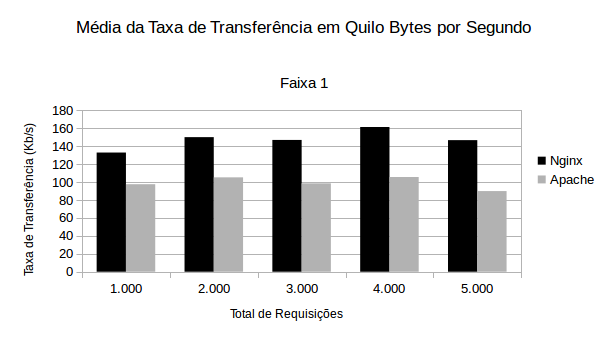
\includegraphics[width=1\linewidth]{graficos/grafico6-f1} 
	\caption{Média da Taxa de Transferência - Faixa 1}
	\label{fig:grafico6-f1}
\end{figure}

\begin{figure}[H]
	\centering
	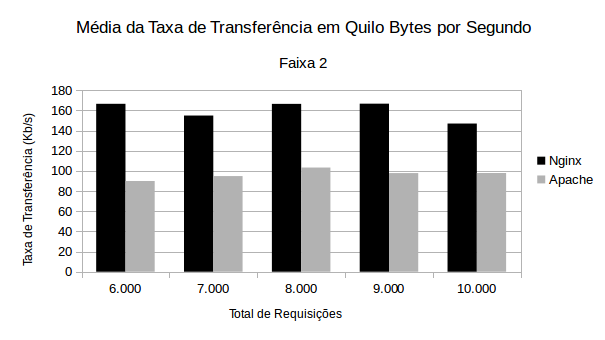
\includegraphics[width=1\linewidth]{graficos/grafico6-f2} 
	\caption{Média da Taxa de Transferência - Faixa 2}
	\label{fig:grafico6-f2}
\end{figure}

\begin{figure}[H]
	\centering
	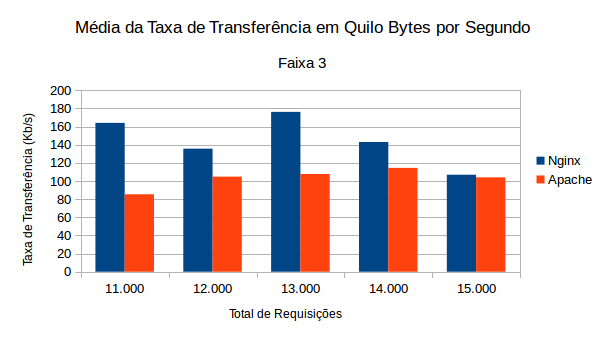
\includegraphics[width=1\linewidth]{graficos/grafico6-f3} 
	\caption{Média da Taxa de Transferência - Faixa 3}
	\label{fig:grafico6-f3}
\end{figure}

\begin{figure}[H]
	\centering
	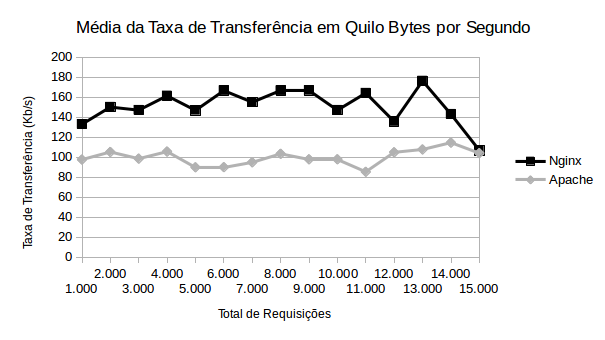
\includegraphics[width=1\linewidth]{graficos/grafico6} 
	\caption{Média da Taxa de Transferência}
	\label{fig:grafico6}
\end{figure}

Nessa métrica, os dois servidores mostraram o desempenho menos discrepante 
entre as métricas analisadas. Entre os quinze valores de requisições testados,  
foram observadas taxas de transferência, em média, 1,52 
vezes maior do que os observados no Apache.

Analisando as três faixas de valores de requisição, as taxas de transferência 
observadas no Nginx foram, em média, 1,48 vezes maior na Faixa 1, 1,43 vezes 
maior na Faixa 2, e 1,42 vezes maior na Faixa 3 comparado com os dados 
mensurados no Apache.